\subsection{Apache Kafka}
\label{sec:kafka}

Apache Kafka ist ein verteiltes Event-Streaming-System.
Die Vermittlung der auftretenden Events läuft in Echtzeit ab.
Kafka basiert auf dem nach dem Publish-Subscribe-Modell.
Events können von Produzenten veröffentlicht werden und Konsumenten können auf diese Events abonnieren.
Durch die Verteilung in einem Cluster kann Kafka den Ausfall einzelner Server ausgleichen.
Zusätzlich können Ströme von Events für einen beliebigen Zeitraum gespeichert werden.

\begin{figure}
    \centering
    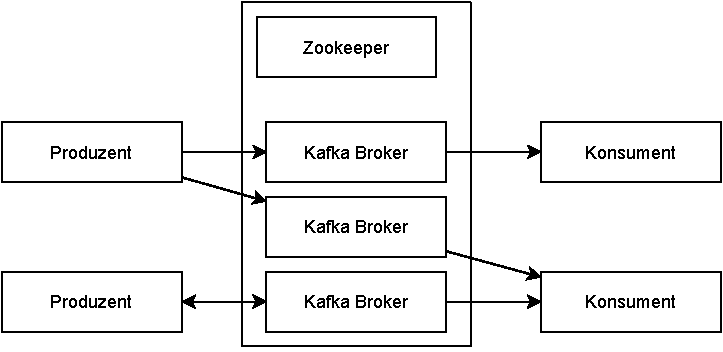
\includegraphics{Grafiken/Grundlagen/Kafka-Cluster.pdf}
    \caption{Kafka-Cluster}
    \label{fig:kafka-cluster}
\end{figure}

Ein Kafka-Cluster (\cref{fig:kafka-cluster}) besteht aus mehreren Brokern, die von Apache Zookeeper verwaltet werden.
Die Broker sind für die Verteilung und Speicherung von Events zuständig.
Mit den Brokern sind die Client-Anwendungen als Produzenten oder Konsumenten verbunden.
Produzenten senden Events an das Cluster und Konsumenten empfangen Events.
Ein Event repräsentiert den Fakt, dass etwas "`passiert"' ist und besteht aus einem Schlüssel, einem Wert, einem Zeitstempel und optionalen Metadaten.
Dabei werden die Werte nicht interpretiert, sondern einfach als Byte-Block versendet und können so eine beliebige Struktur haben.

Events werden in sogenannte Topics unterteilt.
Events in einem Topic können mehrfach gelesen werden und werden nicht nach dem Konsumieren gelöscht.
Es kann aber für jedes Topic eine Dauer festgelegt werden, nach der die Events verworfen werden.
Um ein Topic fehlertolerant zu machen, kann dieses repliziert werden.

Topics werden in Partitionen über verschiedene Broker aufgeteilt, so dass das ganze System gut skalierbar wird.
Ein Produzent kann auch Events auf mehreren Brokern gleichzeitig veröffentlichen.
Wenn ein Event in einem Topic veröffentlicht wird, wird dieses an eine der Partitionen angehängt.
Events, die den gleichen Schlüssel haben, werden immer der gleichen Partition zugeordnet.
Dabei bleibt die Reihenfolge der Events innerhalb einer Partition garantiert erhalten. \parencite{kafka-docs}.

Konsumenten können auch in Gruppen zusammengefasst werden (\cref{fig:kafka-gruppen}).
Innerhalb einer Gruppe werden Events eines Topic innerhalb der Mitglieder, die dieses Topic abonniert haben, aufgeteilt.
Diese Funktion kann zum Beispiel für den Lastausgleich verwendet werden.

\begin{figure}
    \centering
    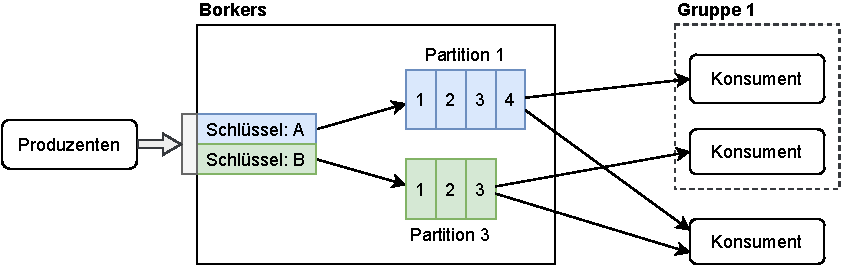
\includegraphics{Grafiken/Grundlagen/Kafka-Gruppen.pdf}
    \caption{Kafka-Gruppen}
    \label{fig:kafka-gruppen}
\end{figure}